\documentclass[11pt]{article}
\usepackage[letterpaper,left=0.82in,right=1.32in,top=0.78in,bottom=0.82in]{geometry}
\usepackage{amsmath,amssymb,mathtools,amsthm}
\usepackage{booktabs,longtable,tabularx,array,multirow}
\usepackage{xcolor,enumitem,hyperref,microtype,fancyhdr}
\usepackage{tikz}
\usetikzlibrary{arrows.meta,positioning,shapes.geometric,fit}
\usepackage[T1]{fontenc}
\usepackage{lmodern}

\definecolor{navy}{RGB}{28,62,102}
\definecolor{bluegray}{RGB}{72,91,113}
\definecolor{paleBlue}{RGB}{235,242,250}
\definecolor{paleGreen}{RGB}{232,246,235}
\definecolor{paleAmber}{RGB}{255,247,224}
\definecolor{paleRed}{RGB}{252,235,235}
\definecolor{darkGreen}{RGB}{30,105,52}
\definecolor{darkAmber}{RGB}{145,91,0}
\definecolor{darkRed}{RGB}{145,35,35}

\hypersetup{colorlinks=true,linkcolor=navy,urlcolor=navy,citecolor=navy,hypertexnames=false,
  pdfauthor={OpenAI},pdftitle={Mortensen-Pissarides (1994) Lean 4 Replication Architecture}}
\pagestyle{fancy}
\fancyhf{}
\lhead{MP (1994): Lean 4 Replication Architecture, v2}
\rhead{\thepage}
\setlength{\headheight}{14pt}
\setlength{\parindent}{0pt}
\setlength{\parskip}{5.5pt}
\setlist[itemize]{leftmargin=1.35em,itemsep=2.2pt,topsep=3pt}
\setlist[enumerate]{leftmargin=1.55em,itemsep=2.5pt,topsep=3pt}
\renewcommand{\arraystretch}{1.12}

\newcommand{\epsd}{\varepsilon_d}
\newcommand{\epsu}{\varepsilon_u}
\newcommand{\E}{\mathbb{E}}
\newcommand{\R}{\mathbb{R}}
\newcommand{\paperloc}[1]{\textbf{Paper location:} #1}
\newcommand{\leanclass}[1]{\textbf{Lean classification:} #1}
\newcommand{\core}{\textcolor{darkGreen}{\textbf{Core Lean proof target}}}
\newcommand{\infra}{\textcolor{darkAmber}{\textbf{Lean target after analytic infrastructure}}}
\newcommand{\finite}{\textcolor{navy}{\textbf{Finite-state Lean specialization}}}
\newcommand{\hybrid}{\textcolor{navy}{\textbf{Hybrid Lean + numerical replication}}}
\newcommand{\outside}{\textcolor{darkRed}{\textbf{Not a core Lean target}}}
\newcommand{\statusbox}[2]{\vspace{2pt}\noindent\colorbox{#1}{\parbox{0.955\linewidth}{\small #2}}\vspace{2pt}}
\newcommand{\resultname}[1]{\medskip\noindent\textbf{#1.}}
\newcommand{\leanname}[1]{\texttt{#1}}

\title{\textbf{Mortensen--Pissarides (1994)}\\[3pt]
\Large A Paper-Centered and Lean-Executable Replication Architecture\\[3pt]
\large Version 2: Economic Contract, Theorem Catalogue, and Proof Roadmap}
\author{Prepared as the governing document for a restarted Lean 4 replication}
\date{July 2026}

\begin{document}
\maketitle

\begin{abstract}
This document reconstructs the intellectual architecture of Mortensen and Pissarides (1994), \emph{Job Creation and Job Destruction in the Theory of Unemployment}, and converts it into an executable Lean 4 proof program. It is deliberately paper-centered: Section 1 uses the paper's symbols, Sections 2--4 reconstruct the analytical core, and Section 7 ranks the theorem targets by economic importance and logical dependency. At the same time, the architecture is designed around what Lean can prove cleanly. The static model is expressed first in probability-measure form, the paper's CDF formulas are recovered as theorems, the graphical uniqueness argument is replaced by an order-theoretic proof, and simulation is separated from deductive verification. The document is a formalization contract, not a report on the legacy repository.
\end{abstract}

\statusbox{paleBlue}{\textbf{Central recommendation.} Restart the intellectual architecture, retain the old repository only as a source of reusable lemmas, and organize the new project around one main analytical package: value equilibrium $\Longleftrightarrow$ a unique reduced steady-state pair $(\theta,\epsd)$, followed by comparative statics. The first implementation milestone is the surplus/cutoff layer; the most important final theorem is the full steady-state characterization and uniqueness theorem.}

\tableofcontents
\newpage

\section*{Executive decision: is this the right replication strategy?}
\addcontentsline{toc}{section}{Executive decision}

Yes. A paper-centered reconstruction is the best option for this paper, provided it is not merely a prose summary. The architecture must simultaneously satisfy three tests:

\begin{enumerate}
\item \textbf{Economic fidelity.} Every object and result must retain the timing, surplus-sharing, free-entry, and endogenous-destruction logic of the paper.
\item \textbf{Logical fidelity.} Equations that define equilibrium must be distinguished from results derived from those equations. In particular, monotonicity, cutoff uniqueness, equations (8), (10), (12), and (13), equilibrium uniqueness, and comparative statics cannot be stored as assumptions.
\item \textbf{Lean executability.} The formal target must be decomposed into lemmas supported by ordered-field algebra, measure theory, continuity, and finite-state dynamics. Numerical calibration and Monte Carlo evidence should not be forced into the theorem-proving core.
\end{enumerate}

The generic formalization workflow proposed for other dynamic economic models should be specialized here. MP (1994) does \emph{not} require a general Bellman-contraction or invariant-measure library before useful progress can be made. The Poisson reset structure and linear flow payoffs collapse the static value system to an affine surplus equation. Lean should exploit this special structure rather than begin with a maximally general dynamic-programming framework.

\begin{center}
\small
\begin{tabularx}{0.95\textwidth}{@{}p{0.23\textwidth}X p{0.22\textwidth}@{}}
\toprule
Paper component & Recommended treatment & Classification \\
\midrule
Section 2 setup and equations (1)--(7) & Encode faithfully as primitives and equilibrium equations; prove algebraic consequences. & \core \\
Section 3 steady state and Appendix & Full formal replication, including corrected existence conditions and comparative statics. & \core / \infra \\
Section 4 two-state shocks & Formalize exact value identities, cutoff/creation equations, and impact asymmetry; qualify informal volatility claims. & \infra / \finite \\
Section 5 equations (32)--(38) & Formalize a finite-state Markov specialization and exact accounting laws. & \finite / \hybrid \\
Calibration, Monte Carlo results, Tables I--II & Reproduce in Python or Julia; Lean may certify inputs, identities, and residual bounds. & \outside \\
\bottomrule
\end{tabularx}
\end{center}

\newpage
\section{Paper-faithful economic setup and notation}

\subsection{Economic environment and timing}

There is a continuum of one-job firms and a fixed labor force normalized to one. A job is either vacant and searching, filled and producing, or destroyed. Workers are either unemployed and searching or employed; there is no on-the-job search.

A filled job with idiosyncratic state $\varepsilon$ produces flow output
\[
 p+\sigma\varepsilon.
\]
The aggregate component is $p$. The parameter $\sigma$ scales dispersion in the job-specific component. Idiosyncratic states are redrawn at Poisson rate $\lambda$ from a distribution $F$. The paper assumes no mass points and finite upper support $\epsu$; it normalizes the draw to mean zero and variance one so that $\sigma$ is the standard deviation of job-specific productivity.

New jobs are created at the upper support $\epsu$. This is an economic assumption, not a consequence of the stochastic process: before creation, technology is flexible, while an existing job's technology is irreversible. After an idiosyncratic redraw, the firm may destroy the match at zero cost. Recruiting is costly because an open vacancy incurs flow cost $c$.

Vacancies and unemployed workers meet through a constant-returns matching function $m(v,u)$. Define market tightness and the two meeting rates by
\[
 \theta=\frac vu,\qquad q(\theta)=\frac{m(v,u)}{v}=m(1,1/\theta),
 \qquad \theta q(\theta)=\frac{m(v,u)}{u}=m(\theta,1).
\]
The paper assumes $q'(\theta)<0$ and that the elasticity of $q$ lies strictly between $-1$ and $0$. Thus vacancies fill more slowly in a tighter market, while workers find jobs faster.

Wages are continuously renegotiated to split total match surplus. The worker receives share $\beta\in(0,1)$ and the firm share $1-\beta$. Vacancies enter until their value is zero.

\statusbox{paleGreen}{\core\quad The setup is a fair Lean target. The right formalization is a continuous idiosyncratic state with a probability measure and a scalar tightness $\theta$. A full two-argument matching function is optional in the core static layer; $q$ and $\theta q(\theta)$ contain all information used in Sections 3--4.}

\subsection{Paper notation}

The economic exposition in this document retains the paper's notation. Lean-normalized identifiers are introduced only in Section 6.

\begin{longtable}{>{\raggedright\arraybackslash}p{0.105\textwidth} >{\raggedright\arraybackslash}p{0.51\textwidth} >{\raggedright\arraybackslash}p{0.26\textwidth}}
\toprule
Symbol & Meaning in the paper & Formal role \\
\midrule
\endfirsthead
\toprule
Symbol & Meaning in the paper & Formal role \\
\midrule
\endhead
$p$ & Aggregate component of labor productivity / product price. & Scalar parameter or aggregate state. \\
$\sigma$ & Scale of idiosyncratic dispersion. & Positive scalar. \\
$\varepsilon$ & Current job-specific productivity component. & Real state variable. \\
$F$ & CDF of a fresh idiosyncratic draw. & Derived from a probability measure. \\
$\epsu$ & Finite upper support; productivity of a newly created job. & Real support bound. \\
$\epsd$ & Endogenous reservation idiosyncratic productivity. & Cutoff / equilibrium unknown. \\
$\lambda$ & Poisson rate of idiosyncratic redraws. & Positive hazard. \\
$\mu$ & Poisson rate of aggregate-state transitions in Section 4. & Positive hazard. \\
$r$ & Discount rate. & Positive scalar. \\
$c$ & Flow vacancy cost. & Positive scalar. \\
$b$ & Flow value of unemployment or leisure. & Scalar. \\
$\beta$ & Worker's share of total match surplus. & Parameter in $(0,1)$. \\
$u$ & Unemployment rate. & Endogenous stock. \\
$v$ & Vacancy rate. & Endogenous stock. \\
$\theta=v/u$ & Market tightness. & Principal static equilibrium variable. \\
$m(v,u)$ & Constant-returns aggregate matching flow. & Matching technology. \\
$q(\theta)$ & Vacancy-filling rate. & Positive decreasing function. \\
$\theta q(\theta)$ & Job-finding rate per unemployed worker. & Positive increasing function under the elasticity condition. \\
$V$ & Asset value of a vacancy. & Scalar value. \\
$J(\varepsilon)$ & Firm's value of a filled job at state $\varepsilon$. & Real-valued function. \\
$W(\varepsilon)$ & Worker's value of employment at state $\varepsilon$. & Real-valued function. \\
$U$ & Worker's value of unemployment. & Scalar value. \\
$w(\varepsilon)$ & Wage paid at state $\varepsilon$. & Transfer function. \\
$S(\varepsilon)$ & Total notional match surplus, $J(\varepsilon)+W(\varepsilon)-U$. & Real-valued function. \\
$\max\{S(\varepsilon),0\}$ & Surplus after the optimal destruction decision. & Active continuation value. \\
$\varepsilon_d(p)$ & State-contingent cutoff in the general Markov model. & Function of aggregate state. \\
$\alpha(p)$ & Worker meeting rate in Section 5. & Function of aggregate state. \\
$n_t(\varepsilon)$ & Employment distribution over idiosyncratic states. & Density in the paper; measure in Lean. \\
\bottomrule
\end{longtable}

\subsection{A crucial distinction: raw versus active surplus}

The paper uses one symbol $S$ in two roles. Equation (8) defines a \emph{notional} surplus that may be negative. When a new idiosyncratic draw arrives, the firm destroys the job if the notional surplus is negative, so the continuation contribution is $\max\{S(x),0\}$.

A sound Lean architecture should preserve the paper notation in the mathematics but distinguish the objects internally:
\[
 S^{\mathrm{raw}}(\varepsilon)=J(\varepsilon)+W(\varepsilon)-U,
 \qquad
 S^{\mathrm{act}}(\varepsilon)=\max\{S^{\mathrm{raw}}(\varepsilon),0\}.
\]
This avoids defining the surplus itself as nonnegative, which would make the reservation rule circular.

\statusbox{paleAmber}{\textbf{Architecture correction.} The destruction threshold must be derived from the sign of the raw surplus. It is not legitimate to assume a cutoff-shaped surplus or define $S$ directly as $\sigma(\varepsilon-\epsd)/(r+\lambda)$ in the primitive model.}

\subsection{Assumptions, organized by their logical role}

\paragraph{Economic primitives.}
\begin{itemize}
\item $r>0$, $\lambda>0$, $c>0$, $\sigma>0$, and $0<\beta<1$.
\item A probability measure $\nu$ on $\R$ represents idiosyncratic redraws; $F(x)=\nu(( -\infty,x])$.
\item $\nu((\epsu,\infty))=0$ and $\int |x|\,d\nu(x)<\infty$.
\item New jobs begin at $\epsu$; destruction is costless; vacancies incur flow cost $c$.
\item $q(\theta)>0$ on $\theta>0$ and is strictly decreasing.
\end{itemize}

\paragraph{Assumptions needed only for selected results.}
\begin{itemize}
\item Atomlessness of $\nu$ is needed for continuity of $F$, clean cutoff probabilities, and some derivative formulas, but not for the affine-surplus theorem.
\item Mean zero and unit variance are normalizations needed for the interpretation of $p$ and $\sigma$, not for the core equilibrium algebra.
\item Continuity of $q$ and a bracketing/range condition are needed for equilibrium existence.
\item Differentiability of $q$ and a nonzero Jacobian are needed for the Appendix-style derivative comparative statics.
\item A density $F'$ is needed only for the paper's density notation in equation (35); the Lean transition law should instead be written directly for measures.
\end{itemize}

\paragraph{Equilibrium conditions, not primitive assumptions.}
Equations (1)--(7), free entry, and Nash sharing are conditions defining a value equilibrium. The following must be derived and therefore cannot appear in an assumptions record: equation (8), affine surplus, existence or uniqueness of $\epsd$, equations (10), (12), and (13), equilibrium uniqueness, and all comparative-static orderings.

\statusbox{paleGreen}{\core\quad This assumption split is Lean-executable and economically minimal. In particular, the base probability layer requires only a finite first moment; stronger distributional assumptions enter later and locally.}

\newpage
\section{Steady-state analytical core: equations, theorems, and proof order}

\subsection{Primitive value system: equations (1)--(7)}

The vacancy equation and free-entry condition are
\begin{align}
 rV&=-c+q(\theta)[J(\epsu)-V], \tag{1}\\
 rV&=0. \tag{2}
\end{align}
Total match surplus and Nash sharing are
\begin{align}
 S(\varepsilon)&=J(\varepsilon)+W(\varepsilon)-U, \tag{3}\\
 W(\varepsilon)-U&=\beta S(\varepsilon). \tag{4}
\end{align}
The firm, worker, and unemployment equations are
\begin{align}
 rJ(\varepsilon)
 &=p+\sigma\varepsilon-w(\varepsilon)
 +\lambda(1-\beta)\int\!\left[\max\{S(x),0\}-S(\varepsilon)\right]dF(x), \tag{5}\\
 rW(\varepsilon)
 &=w(\varepsilon)
 +\lambda\beta\int\!\left[\max\{S(x),0\}-S(\varepsilon)\right]dF(x), \tag{6}\\
 rU&=b+\theta q(\theta)[W(\epsu)-U]. \tag{7}
\end{align}

Equations (1), (3), and (5)--(7) are value relationships. Equations (2) and (4) are equilibrium restrictions. They should be encoded in a \emph{value-equilibrium} structure. They are not theorem conclusions, but neither should they be mixed with reduced-form conditions such as (10) and (13).

\statusbox{paleGreen}{\core\quad These equations are appropriate Lean inputs. Define $S$ from $J,W,U$ rather than storing it as an independent unconstrained function. Define the common reset gain once, so equations (5) and (6) share exactly the same continuation term.}

\subsection{The first derived result: the surplus equation (8)}

Using (3), subtracting (7) from the sum of (5) and (6), and applying the sharing rule (4) gives
\begin{equation}
 (r+\lambda)S(\varepsilon)
 =p+\sigma\varepsilon-b
 +\lambda\int\max\{S(x),0\}\,dF(x)
 -\beta\theta q(\theta)S(\epsu). \tag{8}
\end{equation}

\resultname{Theorem S1: Surplus aggregation}
Every value equilibrium satisfying equations (3)--(7) satisfies equation (8) for all $\varepsilon$.

\paperloc{Section 3, printed pp. 400--401, equation (8).}

\leanclass{\core.}
The proof is mostly ring algebra. The only measure-theoretic fact needed is that the integral of a constant under a probability measure equals that constant. This theorem should be proved before any cutoff object is introduced.

\subsection{Affine surplus without differentiation}

Equation (8) contains $\varepsilon$ only through $\sigma\varepsilon$. Evaluating at $\varepsilon_1$ and $\varepsilon_2$ and subtracting gives
\begin{equation}
 (r+\lambda)\bigl[S(\varepsilon_2)-S(\varepsilon_1)\bigr]
 =\sigma(\varepsilon_2-\varepsilon_1). \tag{S2}
\end{equation}
Therefore
\begin{equation}
 S(\varepsilon_2)-S(\varepsilon_1)
 =\frac{\sigma}{r+\lambda}(\varepsilon_2-\varepsilon_1). \tag{S3}
\end{equation}
This proves directly that $S$ is affine and strictly increasing. It is stronger and formally cleaner than first asserting differentiability and writing $S'(\varepsilon)=\sigma/(r+\lambda)$.

Because an affine function with positive slope has a unique zero on $\R$, define
\[
 \epsd \quad\text{by}\quad S(\epsd)=0.
\]
Then
\begin{equation}
 S(\varepsilon)-S(\epsd)
 =\frac{\sigma(\varepsilon-\epsd)}{r+\lambda}. \tag{12}
\end{equation}
Moreover,
\[
 S(\varepsilon)<0\iff \varepsilon<\epsd,
 \qquad
 S(\varepsilon)\ge 0\iff \varepsilon\ge\epsd.
\]
Since free entry with $c>0$ implies $J(\epsu)>0$, one obtains $S(\epsu)>0$ and therefore $\epsd<\epsu$ in an interior equilibrium.

\resultname{Theorem S2: Affine surplus, unique cutoff, and reservation destruction}
Under $r+\lambda>0$ and $\sigma>0$, equation (8) implies: (i) the surplus-difference identity (S3); (ii) strict monotonicity; (iii) a unique zero $\epsd$; (iv) the reservation destruction rule; and (v) equation (12).

\paperloc{Section 3, printed pp. 401--402, prose after equation (8), equations (9) and (12).}

\leanclass{\core.}
This is the best first substantive proof theorem. It uses no differentiation, no implicit function theorem, and no arbitrary cutoff witness. It is the first place where the model's central economic mechanism is genuinely derived.

\statusbox{paleBlue}{\textbf{First milestone versus main theorem.} The affine-surplus/cutoff theorem is the correct first implementation milestone. It is not, by itself, the paper's main theorem. The main static target is the later equivalence and uniqueness theorem for the entire steady-state equilibrium.}

\subsection{A Lean-friendly measure representation of continuation value}

Let $X\sim\nu$ denote a fresh idiosyncratic draw and define the expected excess above a cutoff
\begin{equation}
 H(d)=\E\bigl[(X-d)_{+}\bigr]
 =\int \max\{x-d,0\}\,d\nu(x). \tag{H}
\end{equation}
By equation (12),
\begin{equation}
 \int \max\{S(x),0\}\,d\nu(x)
 =\frac{\sigma}{r+\lambda}H(\epsd). \tag{S4}
\end{equation}
This measure-form identity should be the primary formal object. It requires only a finite first moment and avoids Stieltjes integration by parts.

If $F(x)=\nu(( -\infty,x])$, $\nu$ is supported on $(-\infty,\epsu]$, and the relevant measurability conditions hold, the layer-cake/tail identity gives
\begin{equation}
 H(d)=\int_d^{\epsu}[1-F(x)]\,dx. \tag{Tail}
\end{equation}
Thus the paper's CDF expression is recovered as a theorem from the more primitive measure representation.

\resultname{Theorem S3: Positive-part expectation and tail-CDF representation}
The affine cutoff formula implies (S4). Under the upper-support and integrability assumptions, $H(d)$ equals the tail integral in (Tail).

\paperloc{Section 3, equation (9), where the paper obtains the tail integral by integration by parts.}

\leanclass{The measure identity (S4) is \core; the CDF-tail equivalence is \infra.}
A specialized proof of (Tail) can use Tonelli's theorem applied to
$\max\{X-d,0\}=\int_d^{\epsu}\mathbf{1}\{X>t\}\,dt$.

\subsection{Job-destruction condition: equation (10)}

Evaluating (8) at $\epsd$, using $S(\epsd)=0$, and substituting (S4) gives the measure-form job-destruction condition
\begin{equation}
 p+\sigma\epsd
 =b+\beta\theta q(\theta)S(\epsu)
 -\frac{\sigma\lambda}{r+\lambda}H(\epsd). \tag{JD-raw}
\end{equation}
Free entry and Nash sharing imply
\[
 q(\theta)(1-\beta)S(\epsu)=c,
 \qquad
 \beta\theta q(\theta)S(\epsu)
 =\frac{\beta c}{1-\beta}\theta.
\]
Hence
\begin{equation}
 p+\sigma\epsd
 =b+\frac{\beta c}{1-\beta}\theta
 -\frac{\sigma\lambda}{r+\lambda}H(\epsd). \tag{JD-$\nu$}
\end{equation}
Using (Tail) recovers the paper's equation
\begin{equation}
 p+\sigma\epsd
 =b+\frac{\beta c}{1-\beta}\frac vu
 -\frac{\sigma\lambda}{r+\lambda}
 \int_{\epsd}^{\epsu}[1-F(x)]\,dx. \tag{10}
\end{equation}

\resultname{Theorem S4: Job-destruction equation}
Every interior value equilibrium satisfies (JD-$\nu$); under the CDF-tail theorem it satisfies equation (10).

\paperloc{Section 3, printed p. 401, equations (9)--(10).}

\leanclass{\core in measure form; \infra in the paper's exact CDF form.}
The formal proof should not block on integration by parts. Prove the economically equivalent expectation equation first and recover (10) afterward.

\subsection{Job-creation condition: equation (13)}

Free entry and equation (1) give $q(\theta)J(\epsu)=c$. Nash sharing gives $J(\epsu)=(1-\beta)S(\epsu)$. Equation (12) gives
\[
 S(\epsu)=\frac{\sigma(\epsu-\epsd)}{r+\lambda}.
\]
Therefore
\begin{equation}
 q(\theta)=\frac{c}{1-\beta}
 \frac{r+\lambda}{\sigma(\epsu-\epsd)}. \tag{13}
\end{equation}

\resultname{Theorem S5: Job-creation equation}
Every interior value equilibrium satisfies equation (13).

\paperloc{Section 3, printed p. 402, equations (1)--(4), (12), and (13).}

\leanclass{\core.}
This is elementary once Theorem S2 is available and should be completed in the same milestone as the job-destruction reduction.

\subsection{The reduced equilibrium and the main static equivalence theorem}

Set
\[
 B=\frac{\beta c}{1-\beta},
 \qquad
 K=\frac{c(r+\lambda)}{(1-\beta)\sigma}.
\]
A reduced steady-state equilibrium is a pair $(\theta,\epsd)$ with $\theta>0$ and $\epsd<\epsu$ satisfying
\begin{align}
 B\theta&=p-b+\sigma\epsd
 +\frac{\sigma\lambda}{r+\lambda}H(\epsd), \tag{R-JD}\\
 q(\theta)&=\frac{K}{\epsu-\epsd}. \tag{R-JC}
\end{align}

The project should prove both directions of the reduction.

\resultname{Theorem S6A: Value equilibrium implies reduced equilibrium}
Every interior solution of equations (1)--(7) induces a pair $(\theta,\epsd)$ satisfying (R-JD) and (R-JC), with the cutoff generated by the raw surplus rather than assumed.

\resultname{Theorem S6B: Reduced equilibrium reconstructs a value equilibrium}
Given a pair satisfying (R-JD) and (R-JC), define
\begin{align*}
 S(\varepsilon)&=\frac{\sigma(\varepsilon-\epsd)}{r+\lambda},\\
 J(\varepsilon)&=(1-\beta)S(\varepsilon),\\
 U&=\frac{b+\beta\theta q(\theta)S(\epsu)}{r},\\
 W(\varepsilon)&=U+\beta S(\varepsilon),\\
 V&=0,
\end{align*}
and define $w(\varepsilon)$ from the worker value equation. Then verify equations (1)--(7). The firm equation follows from the surplus equation and worker equation.

\resultname{Main Static Theorem A: Equivalence of value and reduced equilibrium}
Under the primitive and integrability assumptions, interior value equilibria are equivalent to reduced equilibrium pairs, up to the mechanically reconstructed value and wage objects.

\paperloc{Section 3, printed pp. 400--403. The paper performs the forward reduction but does not explicitly state or prove the converse reconstruction.}

\leanclass{\core.}
This is the most important safeguard against a repository that merely assumes equations (10) and (13). It is also more useful than a general Bellman fixed-point theorem for this paper because the affine surplus formula gives an explicit reconstruction.

\subsection{Existence and uniqueness: replacing the graphical argument with an executable proof}

The paper states that equations (10) and (13) uniquely determine $\theta$ and $\epsd$ and illustrates the claim in Figure 1. A formal theorem needs a proof of both existence and uniqueness.

\subsubsection*{A derivative-free uniqueness argument}

The function $H$ is nonincreasing and one-Lipschitz:
\begin{equation}
 -(d_2-d_1)\le H(d_2)-H(d_1)\le 0
 \qquad(d_2>d_1). \tag{H-Lip}
\end{equation}
Suppose two reduced equilibria satisfy $d_2>d_1$. From (R-JD),
\begin{align*}
 B(\theta_2-\theta_1)
 &=\sigma(d_2-d_1)
 +\frac{\sigma\lambda}{r+\lambda}[H(d_2)-H(d_1)]\\
 &\ge \frac{\sigma r}{r+\lambda}(d_2-d_1)>0.
\end{align*}
Thus $\theta_2>\theta_1$. But (R-JC) implies
\[
 q(\theta_2)=\frac{K}{\epsu-d_2}
 >\frac{K}{\epsu-d_1}=q(\theta_1),
\]
which contradicts strict decrease of $q$. Hence there is at most one pair.

\resultname{Theorem S7: Uniqueness of the reduced steady state}
Under $r,\sigma,c>0$, $0<\beta<1$, finite first moment, and strict decrease of $q$, the reduced system has at most one interior solution.

\leanclass{\core.}
This proof is especially well suited to Lean: it uses order, algebra, and the elementary Lipschitz property of the positive-part expectation. It is stronger and more rigorous than relying on an informal diagram or differentiability.

\subsubsection*{Existence requires a genuine boundary condition}

Define the JD-implied tightness
\begin{equation}
 \theta_{JD}(d)=\frac{1}{B}
 \left[p-b+\sigma d+\frac{\sigma\lambda}{r+\lambda}H(d)\right] . \tag{ThetaJD}
\end{equation}
and the scalar residual
\begin{equation}
 \Phi(d)=q(\theta_{JD}(d))-\frac{K}{\epsu-d}. \tag{Phi}
\end{equation}
The function $\theta_{JD}$ is strictly increasing by the same Lipschitz argument used above. If $q$ is continuous, then $\Phi$ is continuous wherever $\theta_{JD}(d)>0$ and $d<\epsu$. Existence follows from the intermediate value theorem if there are $d_L<d_H<\epsu$ such that
\[
 \theta_{JD}(d)>0\text{ on }[d_L,d_H],
 \qquad \Phi(d_L)\ge 0,\quad \Phi(d_H)\le 0.
\]
A later specialization may replace this explicit bracket by Inada-type range conditions on $q$.

\resultname{Theorem S8: Existence of a reduced steady state}
Under continuity and a transparent bracketing condition, the reduced system has an interior solution.

\resultname{Main Static Theorem B: Unique steady-state equilibrium}
Combining Theorems S6--S8 yields existence and uniqueness of the value equilibrium and its reduced pair.

\paperloc{Section 3, printed p. 402 and Figure 1.}

\leanclass{\core.}
The paper's uniqueness assertion is a fair Lean target, but the published statement is incomplete as an existence theorem. The formal version should be labeled as a corrected theorem with explicit boundary conditions.

\subsection{Unemployment and the Beveridge identity: equation (14)}

At a fixed $(\theta,\epsd)$, employment separates at hazard $\lambda F(\epsd)$ and unemployed workers find jobs at rate $\theta q(\theta)=m(\theta,1)$. Flow balance is
\[
 (1-u)\lambda F(\epsd)=u\theta q(\theta).
\]
Solving gives
\begin{equation}
 u=\frac{\lambda F(\epsd)}{\lambda F(\epsd)+\theta q(\theta)}
 =\frac{\lambda F(\epsd)}{\lambda F(\epsd)+m(v/u,1)}. \tag{14}
\end{equation}

\resultname{Theorem S9: Steady-state unemployment identity}
Flow balance is equivalent to equation (14), provided the denominator is positive.

\paperloc{Section 3, printed p. 403, equation (14).}

\leanclass{\core.}
The identity is elementary. The slope and convexity of the Beveridge curve are not unconditional results: the paper explicitly assumes that the matching effect dominates the endogenous-destruction effect. Lean should encode that dominance condition if a slope theorem is desired.

\subsection{Static theorem package: what should count as replicated?}

The Section 3 static model is replicated only when the following chain is complete:
\[
\begin{array}{c}
\text{equations (1)--(7)}\\
\Downarrow\\
\text{equation (8), affine raw surplus, and unique cutoff}\\
\Downarrow\\
\text{measure-form JD and JC, hence equations (10) and (13)}\\
\Downarrow\\
\text{value/reduced equivalence}\\
\Downarrow\\
\text{existence and uniqueness of }(\theta,\epsd)\\
\Downarrow\\
\text{flow balance and equation (14).}
\end{array}
\]
Merely defining the right-hand sides of (10), (12), or (13), or storing them as fields of an equilibrium structure, does not constitute replication.

\newpage
\section{Comparative statics and the Appendix}

\subsection{Why the comparative statics need two formal layers}

The paper uses two logically different exercises:
\begin{enumerate}
\item \textbf{Partial equilibrium:} vary a parameter while holding $\theta=v/u$ fixed and solve the job-destruction equation for $\epsd$.
\item \textbf{General equilibrium:} allow both $\theta$ and $\epsd$ to move along equations (10) and (13).
\end{enumerate}
A correct Lean development must not combine these statements or reuse a fixed-$\theta$ derivative as a full-equilibrium conclusion.

\subsection{Partial-equilibrium cutoff comparative statics without calculus}

For fixed $\theta$, define
\begin{equation}
 G(d;p,b,\lambda,r,\sigma,\theta)
 =p-b-B\theta+\sigma d
 +\frac{\sigma\lambda}{r+\lambda}H(d). \tag{G}
\end{equation}
The cutoff solves $G(d;\cdot)=0$. The Lipschitz property of $H$ implies $G$ is strictly increasing in $d$ because
\[
 G(d_2)-G(d_1)
 \ge \frac{\sigma r}{r+\lambda}(d_2-d_1)>0.
\]
Therefore root comparisons can be proved by order arguments:

\begin{center}
\begin{tabularx}{0.94\textwidth}{@{}lXl@{}}
\toprule
Change, holding $\theta$ fixed & Reason & Cutoff response \\
\midrule
$p$ rises & $G$ shifts upward & $\epsd$ falls \\
$b$ rises & $G$ shifts downward & $\epsd$ rises \\
$\theta$ rises & $-B\theta$ falls & $\epsd$ rises \\
$\lambda$ rises & $\lambda/(r+\lambda)$ rises and $H\ge0$ & $\epsd$ falls \\
$r$ rises & $\lambda/(r+\lambda)$ falls & $\epsd$ rises \\
$\sigma$ rises & sign depends on $d+\frac{\lambda}{r+\lambda}H(d)$ & conditional \\
\bottomrule
\end{tabularx}
\end{center}

\resultname{Theorem C1: Global partial comparative statics}
At fixed $\theta$, the cutoff is decreasing in $p$, increasing in $b$ and $\theta$, decreasing in $\lambda$, and increasing in $r$. These results can be stated globally, without differentiability, whenever the cutoff root exists.

\paperloc{Section 3, printed pp. 401--402.}

\leanclass{\core.}
This order-theoretic formulation is cleaner than the paper's phrase ``easily established by differentiation'' and substantially reduces analytic overhead.

\subsection{Dispersion at fixed tightness: equation (11)}

The paper differentiates equation (10) with respect to $\sigma$ and obtains
\begin{equation}
 \sigma\frac{\partial\epsd}{\partial\sigma}
 =\frac{(r+\lambda)/\sigma}{r+\lambda F(\epsd)}
 \left(p-b-\frac{\beta c}{1-\beta}\theta\right). \tag{11}
\end{equation}
The sign depends on whether aggregate productivity exceeds the opportunity cost of employment.

A Lean implementation should separate:
\begin{itemize}
\item a theorem deriving the derivative identity from differentiability of the cutoff path and the moving-boundary tail integral; and
\item a short algebraic theorem extracting the sign under the paper's profitability condition.
\end{itemize}

\leanclass{\infra.}
The sign algebra is easy. Deriving the derivative of $H(d)$ or the tail integral requires continuity of $F$ at the cutoff; atomlessness supplies that continuity.

\subsection{Full-equilibrium productivity and unemployment-income effects}

The most important aggregate-productivity comparative statics can be proved without an implicit function theorem.

Consider two equilibria with $p_2>p_1$. If $\varepsilon_{d,2}\ge\varepsilon_{d,1}$, the JD equation and the Lipschitz bound imply $\theta_2>\theta_1$. But the JC equation then implies $\theta_2<\theta_1$, a contradiction. Hence $\varepsilon_{d,2}<\varepsilon_{d,1}$, and JC then gives $\theta_2>\theta_1$. The argument reverses for an increase in $b$.

\resultname{Theorem C2: Aggregate productivity and unemployment income}
For unique interior equilibria,
\[
 p\uparrow\quad\Longrightarrow\quad \theta\uparrow,\ \epsd\downarrow,
\]
while
\[
 b\uparrow\quad\Longrightarrow\quad \theta\downarrow,\ \epsd\uparrow.
\]

\paperloc{Section 3, printed pp. 402--404.}

\leanclass{\core.}
This theorem gives the paper's cleanest aggregate-shock prediction and should be proved before the derivative-heavy Appendix results.

\subsection{Appendix comparative statics for $\lambda$, $r$, and $\sigma$}

The Appendix differentiates the two-equation equilibrium system. It establishes:
\begin{center}
\begin{tabularx}{0.93\textwidth}{@{}lXX@{}}
\toprule
Parameter & $\theta=v/u$ & $\epsd$ \\
\midrule
$\lambda$ increases & decreases & decreases \\
$r$ increases & decreases & ambiguous \\
$\sigma$ increases & increases & positive under a sufficient condition such as $p\ge b$ \\
\bottomrule
\end{tabularx}
\end{center}

The formalization should use two layers.

\paragraph{Layer C3a: derivative algebra conditional on an equilibrium path.}
Assume differentiable functions $\theta(t)$ and $d(t)$ satisfy the reduced equations along a parameter path and that all denominators are nonzero. Derive equations (A1)--(A12) and prove the sign conclusions. This layer verifies the Appendix's actual algebra and is executable with standard calculus lemmas.

\paragraph{Layer C3b: local differentiability of equilibrium.}
Use a two-dimensional implicit-function theorem, or a specialized scalar residual $\Phi$, to show that the unique equilibrium varies differentiably when the Jacobian is nonzero. This is the named analytic closure that justifies Layer C3a.

\resultname{Theorem C3: Appendix comparative statics}
Under the paper's differentiability, elasticity, and nondegeneracy conditions, $\partial\theta/\partial\lambda<0$, $\partial\epsd/\partial\lambda<0$, $\partial\theta/\partial r<0$, the sign of $\partial\epsd/\partial r$ is ambiguous, $\partial\theta/\partial\sigma>0$, and $p\ge b$ is sufficient for $\partial\epsd/\partial\sigma>0$.

\paperloc{Appendix, printed pp. 413--414, equations (A1)--(A12).}

\leanclass{\infra.}
These are central economic results and fair Lean targets, but they should not block the earlier static theorem package. The equilibrium-path differentiability theorem should be a named closure target, never an unexplained assumption hidden in the model primitives.

\subsection{From equilibrium variables to job flows}

Conditional on current unemployment $u$, define
\[
 C=m(v,u)=u\theta q(\theta),
 \qquad
 D=(1-u)\lambda F(\epsd).
\]
If $\theta$ rises, creation rises under the paper's elasticity restriction. If $\epsd$ falls, the destruction probability $F(\epsd)$ falls.

\resultname{Main Comparative-Statics Theorem}
Under the static equilibrium results:
\begin{itemize}
\item a positive aggregate productivity shock ($p\uparrow$ or $b\downarrow$) raises job creation and lowers job destruction;
\item a dispersion increase raises job creation and, under the stated cutoff condition, raises job destruction;
\item an increase in $\lambda$ lowers tightness and its direct destruction effect can be offset by the endogenous fall in the cutoff.
\end{itemize}

\paperloc{Section 3, printed p. 404, together with the Appendix.}

\leanclass{The aggregate-productivity result is \core. The dispersion and $\lambda$ results are \infra because they depend on Theorem C3.}

\statusbox{paleBlue}{\textbf{Headline interpretation.} The paper's static analytical contribution is a sign-comovement result, not yet a statistical correlation theorem: aggregate productivity moves creation and destruction in opposite directions, while dispersion moves them in the same direction. Statistical correlations require a stochastic path and an employment distribution and belong to the later dynamic/numerical layer.}

\newpage
\section{Cyclical shocks: exact analytical targets and informal claims}

\subsection{Two-state aggregate productivity}

Section 4 lets aggregate productivity switch between a low value $p$ and a high value $p^*>p$ at Poisson rate $\mu$. Denote low-state surplus and cutoff by $S,\epsd$ and high-state objects by $S^*,\epsd^*$. The paper analyzes the ordering $\epsd^*\le\epsd$.

Unemployment evolves between aggregate jumps according to
\begin{equation}
 \dot u=(1-u)\lambda F(\epsd)-u\theta q(\theta). \tag{15}
\end{equation}
The state-contingent surplus equations (16)--(18) distinguish three regions:
\begin{enumerate}
\item $\varepsilon\ge\epsd$: the job survives in both aggregate states;
\item $\epsd>\varepsilon\ge\epsd^*$: the job survives only in the boom;
\item $\varepsilon<\epsd^*$: the job is destroyed in either state.
\end{enumerate}

\statusbox{paleGreen}{\finite\quad A two-state aggregate process is a fair and useful Lean target. Use a finite state type and explicit piecewise regions. Do not begin with an arbitrary measurable aggregate-state space.}

\subsection{Piecewise affine surplus}

The paper derives different slopes in the boom-only region and the common-survival region. In particular:
\begin{itemize}
\item for $\varepsilon\ge\epsd$, $\partial S/\partial\varepsilon=\partial S^*/\partial\varepsilon=\sigma/(r+\lambda)$;
\item for $\epsd>\varepsilon\ge\epsd^*$, $\partial S^*/\partial\varepsilon=\sigma/(r+\lambda+\mu)$.
\end{itemize}
Equations (19)--(24) then characterize the boom and recession cutoffs. The economic result is that expected recovery raises the option value of a recession match, while expected downturn lowers the option value of a boom match.

\resultname{Theorem D1: Two-state piecewise surplus and cutoff equations}
Conditional on $\epsd^*\le\epsd$, equations (16)--(18) imply the piecewise affine formulas and the cutoff equations (20) and (24).

\paperloc{Section 4, printed pp. 405--406, equations (16)--(24).}

\leanclass{\infra / \finite.}
The proof is finite-dimensional except for the same positive-part expectation used in the static model. The exact equations are fair targets; the cutoff ordering should be proved separately or made an explicit hypothesis for the regional derivation.

\subsection{Job creation in recession and boom}

From equations (25)--(27), recession surplus satisfies
\begin{equation}
 S(\varepsilon)=\frac{\sigma(\varepsilon-\epsd)}{r+\lambda}, \tag{27}
\end{equation}
so recession job creation obeys
\begin{equation}
 q(\theta)=\frac{c}{1-\beta}
 \frac{r+\lambda}{\sigma(\epsu-\epsd)}. \tag{28}
\end{equation}
The boom surplus formula (29) yields the modified boom creation condition (30). For fixed cutoffs, anticipated switching lowers boom creation relative to the isolated-boom benchmark, while leaving the recession formula in the static form.

\resultname{Theorem D2: State-contingent job-creation equations}
Derive equations (27)--(30) and prove the conditional comparison $\theta^*>\theta$ under the cutoff ordering and positivity conditions used by the paper.

\paperloc{Section 4, printed p. 407, equations (25)--(30).}

\leanclass{\infra / \finite.}
The exact formulas are appropriate proof targets. The broader statement that anticipation ``dampens cyclicality'' must specify a benchmark. A safe theorem compares $\mu>0$ with $\mu=0$ holding cutoffs fixed; a full equilibrium comparison needs additional monotonicity conditions.

\subsection{Impact asymmetry at recession entry}

When the aggregate state falls from $p^*$ to $p$, the cutoff jumps from $\epsd^*$ to $\epsd$. Every existing match with $\varepsilon\in[\epsd^*,\epsd)$ is destroyed immediately. When the aggregate state rises, there is no symmetric instantaneous creation because new employment requires matching.

Let $\eta$ be the current measure of employed matches over idiosyncratic productivity. Then impact destruction at recession entry is
\[
 \eta([\epsd^*,\epsd)).
\]
It is strictly positive exactly when that interval has positive employment mass.

\resultname{Theorem D3: Recession-entry impact asymmetry}
Under $\epsd^*<\epsd$, a boom-to-recession transition generates weakly positive instantaneous destruction equal to the employment mass between the cutoffs, while a recession-to-boom transition generates zero instantaneous creation.

\paperloc{Section 4, printed pp. 407--408.}

\leanclass{\core after an employment-measure layer.}
This is the clean analytical explanation for the paper's asymmetric destruction dynamics. It is more precise and more suitable for Lean than the unqualified statement that destruction is ``more volatile.''

\subsection{What Section 4 does and does not prove}

\begin{center}
\small
\begin{tabularx}{0.95\textwidth}{@{}p{0.38\textwidth}Xp{0.20\textwidth}@{}}
\toprule
Claim & Formal treatment & Status \\
\midrule
Exact equations (16)--(30) & Prove in a two-state finite model. & \infra \\
Anticipation narrows cutoff differences & State with explicit benchmark and prove under ordering/regularity conditions. & \infra \\
Creation is higher in boom than recession & Conditional theorem from (28)--(30). & \infra \\
Recession entry causes immediate destruction & Measure-theoretic impact theorem. & \core \\
Creation and destruction move oppositely under aggregate shocks & Prove statewise rate ordering, not sample correlation. & \core / \infra \\
Destruction is more volatile than creation & Requires a stochastic path, volatility definition, and distribution; paper relies partly on simulation. & \hybrid \\
Destruction leads creation in recessions & Can be formalized as an impact/timing theorem; a statistical lead-lag claim is numerical. & \hybrid \\
\bottomrule
\end{tabularx}
\end{center}

\subsection{Dispersion shocks}

The paper sketches a parallel two-state analysis for $\sigma>\sigma^*$. Its key inequality is
\begin{equation}
 \sigma(\epsu-\epsd)\ge \sigma^*(\epsu-\epsd^*), \tag{31}
\end{equation}
which says that the direct effect of dispersion on job creation dominates the indirect effect through the cutoff. The predicted statewise response is positive comovement: high dispersion raises both creation and destruction.

\resultname{Theorem D4: Dispersion-shock comovement}
Under the Appendix comparative statics and the conditions supporting (31), high dispersion has weakly higher creation and destruction rates than low dispersion.

\paperloc{Section 4, printed pp. 408--409, equation (31).}

\leanclass{\infra.}
The paper only sketches the derivation. The Lean theorem must state the assumptions supporting (31) and should separate steady-state ordering from transition dynamics.

\statusbox{paleAmber}{\textbf{Section 4 replication standard.} A complete analytical replication does not require proving the paper's simulated variance and correlation statistics. It requires the exact two-state equations, conditional cutoff and creation comparisons, and the impact-asymmetry theorem.}

\newpage
\section{General Markov formulation, employment dynamics, and the simulation boundary}

\subsection{General Markov equilibrium: equations (32)--(34)}

Section 5 first states a general Markov version before calibrating. Aggregate productivity is $p$, aggregate jumps arrive at rate $\mu$, and $G(\cdot\mid p)$ is the conditional distribution of the next aggregate state. Equilibrium is characterized by the worker meeting rate $\alpha(p)$, the cutoff $\epsd(p)$, and the raw surplus $S(\varepsilon,p)$:
\begin{align}
 \alpha(p)&=m(\theta(p),1),
 \quad q(\theta(p))(1-\beta)S(\epsu,p)=c, \tag{32}\\
 S(\epsd(p),p)&=0, \tag{33}\\
 [r+\lambda+\mu]S(\varepsilon,p)
 &=p+\sigma\varepsilon-b-\alpha(p)\beta S(\epsu,p)\\
 &\quad+\lambda\int_{\epsd(p)}^{\epsu}S(x,p)\,dF(x)
 +\mu\int\max\{S(\varepsilon,y),0\}\,dG(y\mid p). \tag{34}
\end{align}

These equations define a Markov equilibrium; the paper does not prove a general existence or uniqueness theorem for the three function objects.

\leanclass{\finite first.}
The appropriate target is a finite aggregate-state specialization, where the final integral in (34) is a finite sum. Proving existence for a fully general measurable state space is not required for a faithful replication and should not block the project.

\subsection{Continuous-time analysis versus discrete-time simulation}

The analytical model uses Poisson jump rates $\lambda$ and $\mu$. The simulation section then evolves employment over quarterly periods using coefficients such as $1-\lambda$ and $\lambda$. This is a discrete-time transition specification. The formalization should not silently identify these two objects.

Use separate layers:
\begin{itemize}
\item a continuous-time finite-state surplus system corresponding to (34); and
\item a discrete-time employment transition operator corresponding to equations (35)--(38).
\end{itemize}
Any link between them should be stated as a discretization convention, not as an exact theorem.

\subsection{Employment-distribution law: equation (35)}

The paper writes $n_t(\varepsilon)$ as a density. This is stronger than the earlier assumption that $F$ has no mass points. A more robust Lean object is a finite employment measure $\eta_t$ on idiosyncratic states. The transition should:
\begin{enumerate}
\item retain surviving matches not hit by an idiosyncratic redraw;
\item redraw shocked surviving employment according to $\nu$ and remove draws below the current cutoff;
\item place newly created matches at $\epsu$;
\item remove jobs rendered unprofitable by an aggregate-state cutoff jump.
\end{enumerate}
Equation (35) can then be recovered when $\eta_t$ and $\nu$ admit densities.

\resultname{Theorem M1: Validity of the employment transition}
For a finite aggregate-state path and admissible cutoff, the transition operator maps finite nonnegative employment measures to finite nonnegative employment measures and has the claimed surviving/redrawn decomposition.

\leanclass{\finite / \infra.}
This is a fair Lean theorem. It is better stated for measures than densities.

\subsection{Creation, destruction, and accounting: equations (36)--(38)}

The paper defines
\begin{align}
 C_t&=\alpha(p_t)[1-N_t], \tag{36}\\
 D_t&=\text{impact destruction from a cutoff increase}
 +\text{idiosyncratic-shock destruction}, \tag{37}\\
 N_{t+1}&=N_t+C_t-D_t. \tag{38}
\end{align}

\resultname{Theorem M2: Employment mass accounting}
Given the measure transition, total employment satisfies equation (38), and the two components of destruction in (37) are nonnegative and exhaustive.

\leanclass{\core within the finite simulation layer.}
This is an exact identity and a good verification target. It should be derived from the transition operator rather than separately assumed.

\subsection{Simulation and calibration}

The paper calibrates a three-state Markov chain, a uniform idiosyncratic distribution, a log-linear matching function, and parameters in Table I. It numerically solves equations (32)--(34), reports state-dependent meeting rates and cutoffs, and simulates 100 samples of 66 quarters to produce Table II.

\paragraph{Appropriate numerical tasks.}
\begin{itemize}
\item reconstruct the transition matrix (39), matching function (40), and parameter values;
\item solve the finite nonlinear equilibrium system;
\item verify residuals of equations (32)--(34);
\item simulate equations (35)--(38);
\item reproduce means, standard deviations, correlations, and confidence intervals.
\end{itemize}

\paragraph{Appropriate Lean contributions.}
\begin{itemize}
\item certify that the transition matrix is stochastic;
\item prove positivity and mass bounds of the transition operator;
\item prove equations (36)--(38) from the operator;
\item optionally verify rational interval bounds for reported numerical residuals.
\end{itemize}

\statusbox{paleRed}{\outside\quad Monte Carlo draws, calibration choices, empirical comparison, and approximate moment matching are not core Lean proof obligations. They should be reproduced with numerical software and linked to Lean through exported parameters and residual checks.}

\newpage
\section{Lean-executable model architecture}

\subsection{Foundational choices}

The restarted project should make the following choices explicitly.

\begin{enumerate}
\item \textbf{Continuous idiosyncratic state in the static core.} Use $\varepsilon\in\R$ and a probability measure $\nu$. Do not replace Section 3 by a finite-state approximation.
\item \textbf{Finite aggregate states first.} Use two states for Section 4 and a finite type for the Section 5 Markov specialization. General measurable aggregate states are optional later work.
\item \textbf{Raw surplus is primary.} Define active continuation as the positive part of raw surplus.
\item \textbf{Measure-form JD is canonical.} Formalize $H(d)=\int(x-d)_+d\nu$ before the CDF tail integral. Recover equation (10) as a paper-facing corollary.
\item \textbf{Tightness is the static market variable.} Use $\theta$ directly. Introduce $u$ and $v$ separately only for the Beveridge curve and dynamics.
\item \textbf{No general Bellman contraction is required.} The static value equations admit an explicit affine solution once the reduced pair is known.
\item \textbf{Existence and uniqueness are separate.} Uniqueness follows from monotonicity and the one-Lipschitz property of $H$; existence needs continuity and a bracket or range condition.
\item \textbf{Comparative statics use the least costly valid method.} Prove $p$ and $b$ results by order. Use a named differentiable-equilibrium-path layer for the Appendix signs.
\item \textbf{Simulation stays external.} Lean verifies exact structure and accounting; Python or Julia computes approximate equilibria and moments.
\end{enumerate}

\subsection{Proposed mathematical object hierarchy}

\begin{center}
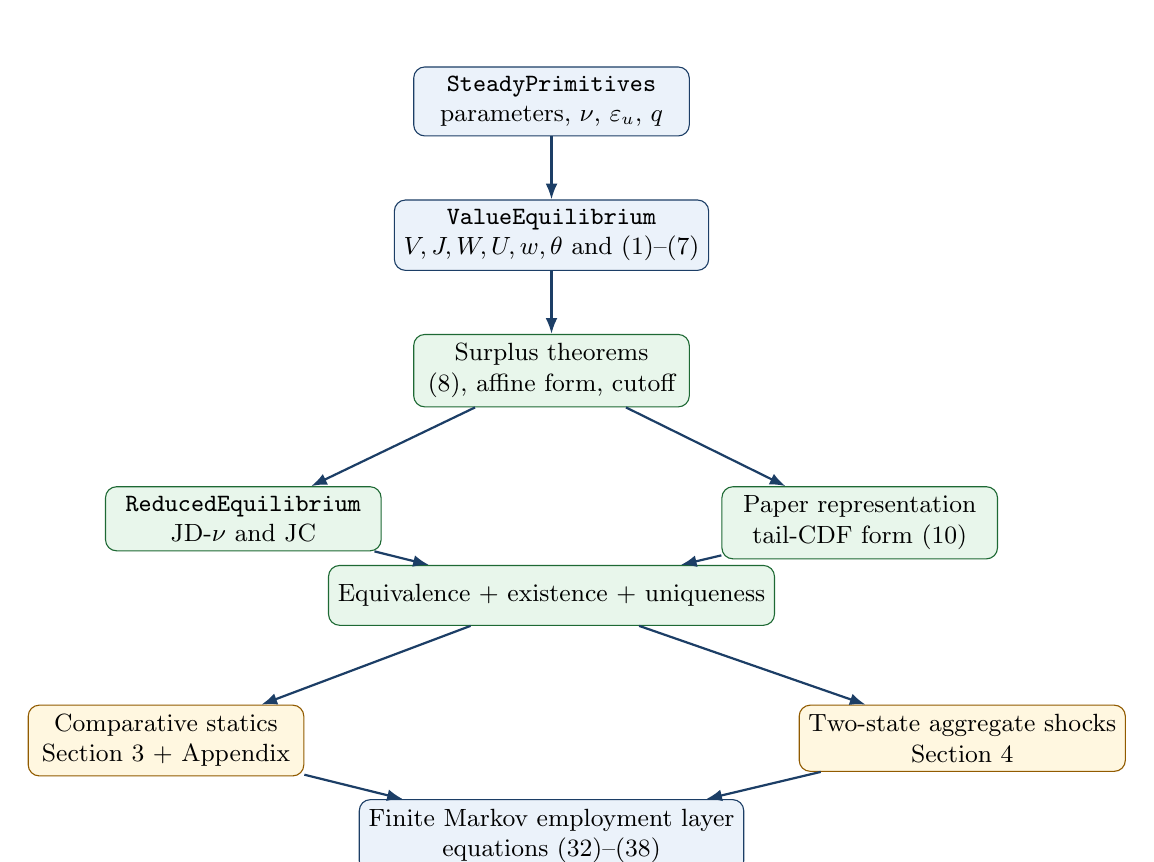
\begin{tikzpicture}[
  node distance=8mm and 11mm,
  every node/.style={font=\small,align=center},
  box/.style={draw=navy,rounded corners,fill=paleBlue,minimum width=3.5cm,minimum height=0.76cm},
  greenbox/.style={draw=darkGreen,rounded corners,fill=paleGreen,minimum width=3.5cm,minimum height=0.76cm},
  amberbox/.style={draw=darkAmber,rounded corners,fill=paleAmber,minimum width=3.5cm,minimum height=0.76cm},
  arr/.style={-{Latex[length=2mm]},thick,navy}]
\node[box] (p) {\texttt{SteadyPrimitives}\\parameters, $\nu$, $\epsu$, $q$};
\node[box,below=of p] (v) {\texttt{ValueEquilibrium}\\$V,J,W,U,w,\theta$ and (1)--(7)};
\node[greenbox,below=of v] (s) {Surplus theorems\\(8), affine form, cutoff};
\node[greenbox,below left=10mm and 4mm of s] (r) {\texttt{ReducedEquilibrium}\\JD-$\nu$ and JC};
\node[greenbox,below right=10mm and 4mm of s] (t) {Paper representation\\tail-CDF form (10)};
\node[greenbox,below=20mm of s] (e) {Equivalence + existence + uniqueness};
\node[amberbox,below left=10mm and 3mm of e] (c) {Comparative statics\\Section 3 + Appendix};
\node[amberbox,below right=10mm and 3mm of e] (d) {Two-state aggregate shocks\\Section 4};
\node[box,below=22mm of e] (m) {Finite Markov employment layer\\equations (32)--(38)};
\draw[arr] (p)--(v);
\draw[arr] (v)--(s);
\draw[arr] (s)--(r);
\draw[arr] (s)--(t);
\draw[arr] (r)--(e);
\draw[arr] (t)--(e);
\draw[arr] (e)--(c);
\draw[arr] (e)--(d);
\draw[arr] (c)--(m);
\draw[arr] (d)--(m);
\end{tikzpicture}
\end{center}

\subsection{Primitive structures: what belongs and what does not}

A conceptual Lean skeleton is:

\begin{verbatim}
structure SteadyPrimitives where
  r lambda c sigma beta b p epsUpper : Real
  shock : Measure Real
  q : Real -> Real
  -- primitive positivity, probability, support, moment, and q assumptions

structure ValueEquilibrium (P : SteadyPrimitives) where
  theta : Real
  V U : Real
  J W wage : Real -> Real
  -- equations (1), (2), (4), (5), (6), (7)

-- Defined, not stored independently:
def surplus (E : ValueEquilibrium P) (eps : Real) : Real :=
  E.J eps + E.W eps - E.U

def activeSurplus (E : ValueEquilibrium P) (eps : Real) : Real :=
  max (surplus E eps) 0

structure ReducedEquilibrium (P : SteadyPrimitives) where
  theta epsCut : Real
  jd_measure : ...
  jc : ...
\end{verbatim}

This is intentionally schematic. The exact Lean code should use existing Mathlib conventions for measures and integrals.

The following must \emph{not} be fields of \texttt{SteadyPrimitives}, \texttt{ValueEquilibrium}, or a general assumptions structure:
\begin{itemize}
\item surplus monotonicity or affinity;
\item existence or uniqueness of $\epsd$;
\item the formula $S(\varepsilon)=\sigma(\varepsilon-\epsd)/(r+\lambda)$;
\item equations (10), (12), or (13) inside the value-equilibrium record;
\item uniqueness of the reduced pair;
\item signs of comparative statics;
\item state ordering such as $\epsd^*\le\epsd$ unless explicitly used as a hypothesis for a conditional regional theorem.
\end{itemize}

\subsection{Expected theorem declarations}

The new project should expose theorem names close to the following conceptual API:

\small
\begin{longtable}{>{\raggedright\arraybackslash}p{0.34\textwidth} >{\raggedright\arraybackslash}p{0.54\textwidth}}
\toprule
Suggested declaration & Mathematical content \\
\midrule
\endfirsthead
\toprule
Suggested declaration & Mathematical content \\
\midrule
\endhead
\leanname{surplus\_equation} & Derive equation (8) from the value-equilibrium fields. \\
\leanname{surplus\_sub} & $S(e_2)-S(e_1)=\sigma(e_2-e_1)/(r+\lambda)$. \\
\leanname{surplus\_strictMono} & Strict monotonicity of raw surplus. \\
\leanname{existsUnique\_cutoff} & Existence and uniqueness of the zero of affine surplus. \\
\leanname{surplus\_eq\_cutoff} & Equation (12). \\
\leanname{activeSurplus\_integral} & Positive-part expectation equals $\sigma H(\epsd)/(r+\lambda)$. \\
\leanname{positivePart\_tail} & $H(d)=\int_d^{\epsu}(1-F)$. \\
\leanname{valueEq\_jdMeasure} & Derive JD-$\nu$. \\
\leanname{valueEq\_jc} & Derive equation (13). \\
\leanname{valueEq\_to\_reducedEq} & Forward equilibrium reduction. \\
\leanname{reducedEq\_to\_valueEq} & Explicit value/wage reconstruction. \\
\leanname{reducedEq\_unique} & Derivative-free uniqueness of $(\theta,\epsd)$. \\
\leanname{reducedEq\_exists} & IVT existence under a bracket. \\
\leanname{steadyState\_equiv} & Main equivalence and unique equilibrium package. \\
\leanname{equilibrium\_mono\_p} & $p\uparrow\Rightarrow\theta\uparrow,\epsd\downarrow$. \\
\leanname{appendix\_lambda\_signs} & Appendix signs for $\lambda$ along a differentiable path. \\
\leanname{twoState\_impact} & Employment mass between old and new cutoffs. \\
\leanname{employment\_massBalance} & Equation (38) from the transition operator. \\
\bottomrule
\end{longtable}
\normalsize

\subsection{Analytic infrastructure, ranked by necessity}

\begin{enumerate}
\item \textbf{Immediate:} probability integral of constants, positive-part measurability, integrability from a finite first moment, and one-Lipschitz properties of $d\mapsto\int(x-d)_+d\nu$.
\item \textbf{Next:} continuity of $H$, continuity of compositions with $q$, and the intermediate value theorem.
\item \textbf{Paper-form bridge:} layer-cake / tail-integral identity and CDF continuity under atomlessness.
\item \textbf{Comparative statics:} derivatives of $H$ at continuity points of $F$, differentiation along equilibrium paths, and a local implicit-function theorem or scalar inverse theorem.
\item \textbf{Dynamic extension:} finite measures, restriction to intervals, finite-state kernels, and total-mass identities.
\end{enumerate}

A general Bellman contraction, measurable selection theorem, Krylov--Bogoliubov theorem, or invariant-law uniqueness result is not on the critical path for this paper.

\subsection{Proposed file structure}

\begin{verbatim}
MP1994v2/
  Primitives.lean
  ValueEquilibrium.lean
  Surplus.lean
  PositivePart.lean
  TailCDF.lean
  ReducedEquilibrium.lean
  Reconstruction.lean
  SteadyStateExistence.lean
  Unemployment.lean
  ComparativeStaticsOrder.lean
  ComparativeStaticsDiff.lean
  TwoState.lean
  DispersionState.lean
  EmploymentMeasure.lean
  FiniteMarkov.lean
  SimulationAccounting.lean
  Audit.lean

docs/
  replication_architecture_v2.tex
  replication_architecture_v2.pdf
  theorem_status.tex
  theorem_status.pdf
numerics/
  solve_markov_equilibrium.py
  reproduce_simulation.py
  residual_report.json
\end{verbatim}

\newpage
\section{Prioritized theorem roadmap}

\subsection{Which results are the key theorems of the paper?}

The paper contains no formally numbered propositions. Its contributions are spread across equations, diagrams, Appendix calculations, and prose. The replication should therefore identify theorem \emph{packages} rather than count every numbered equation as a theorem.

There are two different meanings of ``key theorem'':

\begin{itemize}
\item \textbf{Main analytical theorem of the static model:} the value system has an endogenous reservation rule and is equivalent to a unique reduced equilibrium pair $(\theta,\epsd)$ satisfying job destruction and job creation conditions.
\item \textbf{Headline economic theorem of the paper:} aggregate productivity shocks move job creation and destruction in opposite directions, while dispersion shocks move them in the same direction; anticipated shocks also create asymmetric destruction dynamics.
\end{itemize}

The first is the foundational theorem Lean should establish. The second is the economic payoff built on top of it.

\subsection{Ranked theorem catalogue}

\small
\begin{longtable}{>{\raggedright\arraybackslash}p{0.045\textwidth} >{\raggedright\arraybackslash}p{0.23\textwidth} >{\raggedright\arraybackslash}p{0.16\textwidth} >{\raggedright\arraybackslash}p{0.32\textwidth} >{\raggedright\arraybackslash}p{0.12\textwidth}}
\toprule
Rank & Theorem package & Paper section & Exact target and role & Lean fit \\
\midrule
\endfirsthead
\toprule
Rank & Theorem package & Paper section & Exact target and role & Lean fit \\
\midrule
\endhead
1 & Steady-state representation and equilibrium equivalence & Section 3, eqs. (1)--(13) & Derive (8), affine surplus, unique cutoff, JD/JC, and prove value equilibrium $\Longleftrightarrow$ reduced pair. This is the core economic architecture. & \core \\
2 & Existence and uniqueness of the steady state & Section 3, Figure 1 & Prove at most one pair by order/Lipschitz arguments and existence under explicit boundary conditions. Corrects the paper's informal graphical assertion. & \core \\
3 & Aggregate productivity comparative statics & Section 3 & Prove $p\uparrow$ or $b\downarrow$ implies $\theta\uparrow$, $\epsd\downarrow$, creation up, destruction down. Central and derivative-free. & \core \\
4 & Appendix comparative statics & Section 3 + Appendix, A1--A12 & Prove $\lambda$, $r$, and $\sigma$ sign results using a differentiable equilibrium path and nonzero Jacobian. & \infra \\
5 & Aggregate versus dispersion comovement & Sections 3--4 & Aggregate productivity: creation/destruction move oppositely. Dispersion: both rise under the paper's sufficient conditions. This is the headline mechanism. & \core / \infra \\
6 & Two-state surplus and cutoff characterization & Section 4, eqs. (16)--(30) & Prove piecewise affine surplus, boom/recession cutoff equations, and state-contingent JC conditions. & \finite / \infra \\
7 & Recession-entry impact asymmetry & Section 4 & Prove immediate destruction equals employment mass between cutoffs and has no symmetric boom creation counterpart. & \core after measures \\
8 & Steady-state unemployment and flow balance & Section 3, eq. (14) & Prove Beveridge identity and flow implications, while keeping slope claims conditional. & \core \\
9 & Finite Markov equilibrium representation & Section 5, eqs. (32)--(34) & Encode and analyze a finite aggregate-state version; general existence is not required by the paper. & \finite \\
10 & Employment transition and accounting & Section 5, eqs. (35)--(38) & Prove valid measure transition, creation/destruction decomposition, and mass balance. & \finite / \core \\
11 & Calibration and simulated moments & Section 5, Tables I--II & Reproduce numerically and verify residuals; not a mathematical proof target. & \hybrid \\
\bottomrule
\end{longtable}
\normalsize

\subsection{Dependency-ordered implementation milestones}

\paragraph{Milestone 0: Archive and clean restart.}
Create a new branch or directory. Preserve the legacy project unchanged. Introduce only the primitive structures, value equations, raw surplus definition, and probability assumptions. No reduced conditions or theorem conclusions may be stored as fields.

\textbf{Paper location:} Section 2 and Section 3, equations (1)--(7). \\
\textbf{Difficulty:} low to moderate. \\
\textbf{Completion test:} the value-equilibrium record can state the paper equations without assuming a cutoff or affine surplus.

\paragraph{Milestone 1: Surplus and cutoff layer.}
\begin{itemize}
\item Derive equation (8).
\item Prove the surplus-difference identity.
\item Prove affine surplus, strict monotonicity, unique zero, reservation destruction, and equation (12).
\item Prove $\epsd<\epsu$ from free entry in an interior equilibrium.
\end{itemize}

\textbf{Paper location:} Section 3, equations (3)--(8), prose after (8), and equation (12). \\
\textbf{Difficulty:} elementary to moderate. \\
\textbf{Why first:} this is the first genuine economic theorem and prevents every later cutoff result from being circular.

\paragraph{Milestone 2: Positive-part expectation and reduced equations.}
\begin{itemize}
\item Define $H(d)=\int(x-d)_+d\nu$.
\item Prove measurability, integrability, monotonicity, continuity, and one-Lipschitzness.
\item Derive the active-surplus integral, JD-$\nu$, and JC.
\item Recover equation (10) through a separate tail-CDF theorem.
\end{itemize}

\textbf{Paper location:} Section 3, equations (9)--(13). \\
\textbf{Difficulty:} moderate. \\
\textbf{Completion test:} every value equilibrium produces a reduced pair, with no reduced equation assumed.

\paragraph{Milestone 3: Reconstruction and equivalence.}
Construct $S,J,W,U,V,w$ from a reduced pair and verify equations (1)--(7). Package the two directions as the main equivalence theorem.

\textbf{Paper location:} Section 3. \\
\textbf{Difficulty:} moderate. \\
\textbf{Importance:} highest. This is the point at which the project becomes a formal replication rather than a library of conditional identities.

\paragraph{Milestone 4: Existence and uniqueness.}
\begin{itemize}
\item Prove uniqueness using the Lipschitz JD argument and strict decrease of $q$.
\item Prove existence from continuity and an explicit bracket.
\item Add an optional corollary using standard Inada/range conditions on $q$.
\end{itemize}

\textbf{Paper location:} Section 3, Figure 1. \\
\textbf{Difficulty:} moderate. \\
\textbf{Completion test:} a corrected theorem states exactly when the paper's claimed unique equilibrium exists.

\paragraph{Milestone 5: Core comparative statics.}
First prove fixed-$\theta$ monotone results and the full-equilibrium $p,b$ theorem by order. Then derive creation/destruction responses and equation (14).

\textbf{Paper location:} Section 3, printed pp. 401--404. \\
\textbf{Difficulty:} moderate. \\
\textbf{Economic payoff:} the negative comovement response to aggregate productivity.

\paragraph{Milestone 6: Appendix derivative comparative statics.}
Formalize derivative identities along equilibrium paths, prove A1--A12, and subsequently discharge the local differentiability closure through an implicit-function or scalar inverse theorem.

\textbf{Paper location:} Appendix, printed pp. 413--414. \\
\textbf{Difficulty:} substantial but contained. \\
\textbf{Economic payoff:} $\lambda$, $r$, and $\sigma$ results and dispersion comovement.

\paragraph{Milestone 7: Two-state aggregate shocks.}
Formalize equations (15)--(30), piecewise surplus, cutoff equations, and conditional creation comparisons. Add the employment-measure impact-asymmetry theorem.

\textbf{Paper location:} Section 4, printed pp. 405--408. \\
\textbf{Difficulty:} substantial. \\
\textbf{Scope limit:} do not claim a theorem about unconditional volatility unless a full stochastic metric is defined.

\paragraph{Milestone 8: Finite Markov and numerical interface.}
Implement a finite aggregate-state version of equations (32)--(34), the measure transition behind (35), and accounting (36)--(38). Export a machine-readable parameter schema to numerical code.

\textbf{Paper location:} Section 5, printed pp. 409--412. \\
\textbf{Difficulty:} moderate for accounting, high for nonlinear equilibrium existence. \\
\textbf{Scope limit:} numerical solution and Monte Carlo replication remain external.

\subsection{What should be proved first, and what is the ultimate target?}

\statusbox{paleGreen}{\textbf{First Lean theorem package:} derive equation (8), prove affine raw surplus, prove the unique cutoff and reservation rule, and derive equation (12). This is larger and more meaningful than proving equation (12) for a separately defined closed-form function.}

\statusbox{paleBlue}{\textbf{Ultimate static theorem:} under explicit primitive, continuity, integrability, and boundary conditions, there exists a unique interior value equilibrium; it is equivalent to the unique pair $(\theta,\epsd)$ satisfying JD-$\nu$ and JC, and it generates unemployment through equation (14).}

\statusbox{paleAmber}{\textbf{Ultimate economic theorem:} aggregate productivity shifts creation and destruction in opposite directions, while dispersion shifts them in the same direction under the paper's sufficient conditions; anticipated aggregate shocks additionally generate asymmetric impact destruction.}

\subsection{Fairness to Lean by paper section}

\begin{longtable}{>{\raggedright\arraybackslash}p{0.16\textwidth} >{\raggedright\arraybackslash}p{0.42\textwidth} >{\raggedright\arraybackslash}p{0.29\textwidth}}
\toprule
Paper section & Fair Lean burden & Unfair or unnecessary burden \\
\midrule
\endfirsthead
\toprule
Paper section & Fair Lean burden & Unfair or unnecessary burden \\
\midrule
\endhead
Section 2 & Encode primitives, timing, support, matching rates, and bargaining restrictions. & Formalize empirical motivation or cited historical facts. \\
Section 3 & Full derivation, equilibrium equivalence, existence/uniqueness, flow balance, and comparative statics. & Treat diagrams alone as proofs or assume comparative-static signs. \\
Appendix & Verify derivative identities and sign algebra; eventually justify differentiable equilibrium paths. & Require a universal implicit-function library before any static result can be proved. \\
Section 4 & Prove finite two-state equations and impact asymmetry. & Prove vague words such as ``likely'' or ``more cyclical'' without a formal metric. \\
Section 5 analytical part & Prove finite-state equilibrium equations and exact employment accounting. & Begin with arbitrary measurable aggregate states or density assumptions not used elsewhere. \\
Section 5 simulation & Check matrix validity, identities, and numerical residual certificates. & Reproduce Monte Carlo sampling and moment matching inside Lean. \\
\bottomrule
\end{longtable}

\newpage
\section{Migration, synchronization, and verification protocol}

\subsection{Treatment of the legacy repository}

The existing project should be preserved as an archived branch or directory. It may contain useful algebraic lemmas, notation, and build infrastructure, but no declaration should be migrated merely because it compiles.

For each candidate declaration, ask:
\begin{enumerate}
\item Does its statement correspond to a theorem in this architecture?
\item Are all assumptions primitive or named analytic closures?
\item Is the economic conclusion derived, rather than included as a structure field or theorem hypothesis?
\item Is the theorem at the correct generality: continuous static state, finite aggregate state, or numerical witness?
\item Can its proof be placed in the dependency order of Section 7?
\end{enumerate}

Declarations that define a closed-form surplus or reduced equilibrium formula may be retained as auxiliary definitions, but they cannot substitute for the theorems deriving those formulas from the value system.

\subsection{Synchronized human-readable proof document}

After implementation begins, maintain a separate theorem-status document synchronized with Lean. Each theorem entry should contain:
\begin{itemize}
\item architecture theorem ID and paper location;
\item exact mathematical statement;
\item exact Lean declaration name;
\item primitive assumptions and named closure assumptions;
\item readable proof outline;
\item dependencies;
\item status: green, amber, or red;
\item any difference from the published statement.
\end{itemize}

The architecture document should remain stable. The theorem-status document is the changing progress ledger.

\subsection{Adequacy colors}

\begin{center}
\begin{tabularx}{0.94\textwidth}{@{}p{0.12\textwidth}X@{}}
\toprule
Status & Meaning \\
\midrule
\textcolor{darkGreen}{\textbf{Green}} & The Lean theorem matches the paper or an explicitly corrected statement, derives its conclusion from legitimate inputs, has no \texttt{sorry}, and appears in the readable proof ledger. \\
\textcolor{darkAmber}{\textbf{Amber}} & The theorem is proved conditional on a named analytic closure, or only in a clearly labeled finite-state specialization, or the paper-facing CDF form remains to be derived from a measure-form theorem. \\
\textcolor{darkRed}{\textbf{Red}} & The result is absent, circular, materially weaker without disclosure, based on an arbitrary witness, or still only an equilibrium/assumptions field. \\
\bottomrule
\end{tabularx}
\end{center}

\subsection{Mechanical verification after every milestone}

\begin{enumerate}
\item Run the targeted Lean file and then the project build.
\item Apply \texttt{assert\_no\_sorry} to every new theorem.
\item Print transitive axioms for main theorem packages.
\item Search for prohibited patterns: conclusions in assumptions, hard-coded cutoff formulas in primitive records, or theorem hypotheses that already contain the desired ordering.
\item Check that every green theorem appears in the theorem-status document and every cited Lean name exists.
\item Compile and visually inspect the PDF proof ledger.
\item At major milestones, rerun a dependency audit to ensure that no later result has leaked into an earlier layer.
\end{enumerate}

\subsection{Definition of project completion}

The static replication is complete when Main Static Theorems A and B, Theorems C1--C3, and Theorem S9 are green or transparently amber only for a named and narrowly stated analytic closure. The dynamic analytical replication is complete when Theorems D1--D3 and M1--M2 are established in the finite-state/measure framework. Numerical replication is complete separately when the solver and simulation reproduce the paper's reported system and document residuals and stochastic variation.

\section{Conclusion}

The appropriate formalization of MP (1994) is neither a line-by-line encoding of forty numbered equations nor a generic dynamic-programming project. The paper has a compact mathematical spine:
\[
\begin{array}{c}
\text{value equations}\\
\Downarrow\\
\text{affine raw surplus and endogenous cutoff}\\
\Downarrow\\
\text{JD and JC reduced system}\\
\Downarrow\\
\text{unique steady-state equilibrium}\\
\Downarrow\\
\text{comparative statics and flow comovement}\\
\Downarrow\\
\text{two-state impact asymmetry}.
\end{array}
\]

Lean is well suited to this spine. Its strongest contribution is to force the paper's informal graphical and derivative arguments into explicit assumptions and exact theorem statements. The architecture should exploit the positive-part expectation representation, derivative-free uniqueness, and explicit value reconstruction. Simulation and empirical moment matching should remain in numerical software, linked to Lean through certified equations and accounting identities.

The restarted project should therefore begin with the surplus/cutoff milestone, but it should be governed by the larger objective: a proved equivalence between the original value equilibrium and a unique reduced equilibrium, followed by the paper's principal comparative statics.

\appendix
\newpage
\section{Equation-by-equation role and Lean treatment}

\small
\begin{longtable}{>{\raggedright\arraybackslash}p{0.09\textwidth} >{\raggedright\arraybackslash}p{0.30\textwidth} >{\raggedright\arraybackslash}p{0.34\textwidth} >{\raggedright\arraybackslash}p{0.14\textwidth}}
\toprule
Equation & Economic role & Formal treatment & Classification \\
\midrule
\endfirsthead
\toprule
Equation & Economic role & Formal treatment & Classification \\
\midrule
\endhead
(1) & Vacancy Bellman equation & Field of value equilibrium. & Assumption / definition \\
(2) & Free entry & Field of interior value equilibrium. & Equilibrium condition \\
(3) & Surplus definition & Lean definition from $J,W,U$. & Definition \\
(4) & Nash sharing & Field of value equilibrium. & Equilibrium condition \\
(5)--(7) & Firm, worker, unemployment values & Fields of value equilibrium with common continuation term. & Assumption / definition \\
(8) & Aggregated surplus equation & Derive from (3)--(7). & \core \\
(9) & Tail-integral representation & First prove measure positive-part form; recover CDF form. & \infra \\
(10) & Job-destruction condition & Derive from cutoff, free entry, and (9). & \core / \infra \\
(11) & Fixed-$\theta$ dispersion derivative & Derive after differentiability of $H$ and cutoff path. & \infra \\
(12) & Affine surplus around cutoff & Corollary of surplus-difference theorem. & \core \\
(13) & Job-creation condition & Derive from free entry and (12). & \core \\
(14) & Steady-state unemployment & Derive from flow balance. & \core \\
(15) & Unemployment law of motion & Define/derive from inflow and outflow hazards. & \core \\
(16)--(18) & Two-state surplus equations & Fields of two-state value equilibrium; derive consequences. & \finite \\
(19)--(24) & Piecewise surplus and cutoff equations & Derive conditionally on cutoff ordering. & \infra \\
(25)--(30) & Two-state creation formulas & Derive from two-state surplus and free entry. & \infra \\
(31) & Dispersion dominance inequality & Prove under explicit comparative-static assumptions. & \infra \\
(32)--(34) & General Markov equilibrium characterization & Encode finite-state specialization; no general existence claim required. & \finite \\
(35) & Employment-distribution transition & Replace density notation by a measure transition, then recover density form. & \finite / \infra \\
(36)--(38) & Creation, destruction, mass accounting & Derive from transition operator. & \core in finite layer \\
(39)--(42) & Calibrated Markov chain, matching form, numerical solution & Reproduce numerically; optionally certify matrix and residuals. & \hybrid \\
(A1)--(A12) & Appendix derivative calculations & Two-layer proof: path derivative algebra, then local differentiability closure. & \infra \\
\bottomrule
\end{longtable}
\normalsize

\section{Theorem-status template for future updates}

\small
\begin{longtable}{>{\raggedright\arraybackslash}p{0.09\textwidth} >{\raggedright\arraybackslash}p{0.22\textwidth} >{\raggedright\arraybackslash}p{0.22\textwidth} >{\raggedright\arraybackslash}p{0.12\textwidth} >{\raggedright\arraybackslash}p{0.22\textwidth}}
\toprule
ID & Paper result & Lean declaration & Status & Missing foundation / note \\
\midrule
\endfirsthead
\toprule
ID & Paper result & Lean declaration & Status & Missing foundation / note \\
\midrule
\endhead
S1 & Surplus equation (8) & -- & Red & Implement from value equilibrium. \\
S2 & Affine surplus, cutoff, (12) & -- & Red & Depends on S1. \\
S3 & Positive-part and tail identity & -- & Red & Measure lemmas. \\
S4 & JD condition (10) & -- & Red & Depends on S2--S3 and free entry. \\
S5 & JC condition (13) & -- & Red & Depends on S2 and free entry. \\
S6 & Value/reduced equivalence & -- & Red & Forward and reconstruction directions. \\
S7--S8 & Unique existing steady state & -- & Red & Lipschitz uniqueness, IVT bracket. \\
S9 & Unemployment identity (14) & -- & Red & Flow balance. \\
C1--C2 & Order comparative statics & -- & Red & Depends on unique reduced equilibrium. \\
C3 & Appendix signs & -- & Red & Differentiable equilibrium path. \\
D1--D2 & Two-state equations & -- & Red & Finite aggregate-state value layer. \\
D3 & Impact asymmetry & -- & Red & Employment measure. \\
M1--M2 & Markov transition and accounting & -- & Red & Finite-state transition operator. \\
\bottomrule
\end{longtable}
\normalsize

\section*{Source}
\addcontentsline{toc}{section}{Source}
Dale T. Mortensen and Christopher A. Pissarides, ``Job Creation and Job Destruction in the Theory of Unemployment,'' \emph{Review of Economic Studies} 61(3), 1994, pp. 397--415.

\end{document}
